\documentclass[letterpaper,11pt]{article}
\usepackage{graphicx}
\usepackage{latexsym}
\usepackage[empty]{fullpage}
\usepackage{titlesec}
\usepackage{marvosym}
\usepackage[usenames,dvipsnames]{color}
\usepackage{verbatim}
\usepackage{enumitem}
\usepackage[hidelinks]{hyperref}
\usepackage{fancyhdr}
\usepackage[english]{babel}
\usepackage{tabularx}
\usepackage{fontawesome5}
\usepackage{smartdiagram}
\usepackage{multicol}
\usepackage{lmodern}
\usepackage[most]{tcolorbox}
\usepackage{tikz}
\usetikzlibrary{matrix}



\setlength{\multicolsep}{-3.0pt}
\setlength{\columnsep}{-1pt}
\input{glyphtounicode}
\pagestyle{fancy}
\fancyhf{} % clear all header and footer fields
\fancyfoot{}
\renewcommand{\headrulewidth}{0pt}
\renewcommand{\footrulewidth}{0pt}

% Adjust margins
\addtolength{\oddsidemargin}{-0.6in}
\addtolength{\evensidemargin}{-0.5in}
\addtolength{\textwidth}{1.19in}
\addtolength{\topmargin}{-.7in}
\addtolength{\textheight}{1.4in}
\urlstyle{same}
\raggedbottom
\raggedright
\setlength{\tabcolsep}{0in}

% Sections formatting
\titleformat{\section}{
  \vspace{-7pt}\scshape\raggedright\large\bfseries
}{}{0em}{}[\color{black}\titlerule \vspace{0pt}]

% Ensure that generate pdf is machine readable/ATS parsable
\pdfgentounicode=1

%%%%%%%%%%%%%%%%%%%%%%%%%%%%  Commands  %%%%%%%%%%%%%%%%%%%%%%%%%%%%
\newcommand{\resumeItem}[1]{
  \item\small{
    {#1 \vspace{-3pt}}
  }
}
\newcommand{\resumeSubheading}[4]{
  \vspace{-3pt}\item
    \begin{tabular*}{1.0\textwidth}[t]{l@{\extracolsep{\fill}}r}
      \textbf{#1} & \textbf{\small #2} \\
      \textit{\small#3} & \textit{\small #4} \\
    \end{tabular*}\vspace{-7pt}
}
\newcommand{\resumeSubheadingContinue}[2]{
  \vspace{-3pt}
    \begin{tabular*}{1.0\textwidth}[t]{l@{\extracolsep{\fill}}r}
      \textit{\small#1} & \textit{\small #2} \\
    \end{tabular*}\vspace{-7pt}
}
\newcommand{\resumeProjectHeading}[2]{
  \vspace{-3pt}\item
    \begin{tabular*}{1.0\textwidth}[t]{l@{\extracolsep{\fill}}r}
      \textbf{#1} & \textbf{\small #2} \\
    \end{tabular*}\vspace{-7pt}
}
\newcommand{\resumeSubItem}[1]{\resumeItem{#1}\vspace{0pt}}
\renewcommand\labelitemi{$\vcenter{\hbox{\tiny$\bullet$}}$}
\renewcommand\labelitemii{$\vcenter{\hbox{\tiny$\bullet$}}$}
\newcommand{\resumeSubHeadingListStart}{\begin{itemize}[leftmargin=0.0in, label={}]}
\newcommand{\resumeSubHeadingListEnd}{\end{itemize}}
\newcommand{\resumeItemListStart}{\begin{itemize}}
\newcommand{\resumeItemListEnd}{\end{itemize}\vspace{0pt}}


%four boxes with technologies lists
\tikzstyle{tikzbox} = [draw=black, very thick, rectangle, inner xsep=10pt, inner ysep=10pt, minimum height=40mm, minimum width=40mm, text width=40mm-2*\pgfkeysvalueof{/pgf/inner xsep}]

%diagram of tags with description at bottom, cool graphic with symbols (fontawesome)
\newtcolorbox{mybox}[4][]{%
        enhanced, width=7.75cm, height=1.75cm,
        fontupper=\small\sffamily,
        fonttitle=\large\sffamily\bfseries\slshape,
        leftupper=1.5cm,
        colback=white,
        colframe=white,
        colupper=white,
        title=#2,
        attach title to upper={\\},
        underlay={\fill[#4] (frame.north west)--([xshift=-5mm]frame.north east)--(frame.east)--([xshift=-5mm]frame.south east)-|cycle;},
        overlay={\node[circle, minimum size=2cm, line width=1mm, draw=white, fill=#4, font=\Huge, text=white] at (frame.west) {#3};},
        #1, }

%%%%%%%%%%%%%%%%%%%%%%%%%%%%  Heading  %%%%%%%%%%%%%%%%%%%%%%%%%%%%
\begin{document}
    \begin{center}
        % NAME
        {\Huge\scshape Jason J. Evans} 
        % SUBHEADING
        \\Bioinformatics Engineering and Data Science\\
        \small
        % EMAIL
        \href{mailto:jason.j.evans@gmail.com}{\raisebox{-0.2\height}\faEnvelope\  \underline{jason.j.evans@gmail.com}} ~ 
        % LINKEDIN
        \href{https://www.linkedin.com/in/jasonjevans/}{\raisebox{-0.2\height}\faLinkedin\ \underline{linkedin.com/in/jasonjevans}}  ~
        % GITHUB
        \href{https://github.com/jjevans}{\raisebox{-0.2\height}\faGithub\ \underline{github.com/jjevans}} ~
		%phone
		\href{tel:12624420503}{\raisebox{-0.2\height}\faPhone\ \underline{262-442-0503}}
    \end{center}

%%%%%%%%%%%%%%%%%%%%%%%%%%%%  Education  %%%%%%%%%%%%%%%%%%%%%%%%%%%%


\section{\Large{Highlights}}
    \vspace{-7pt}
%thin outline box
	\fbox{\parbox{\linewidth}{

\begin{minipage}{-0.0\linewidth}
%image to left side of highlights
%        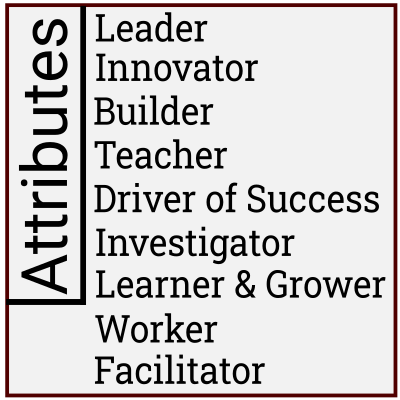
\includegraphics[scale=0.45]{resume_attributes.png}
        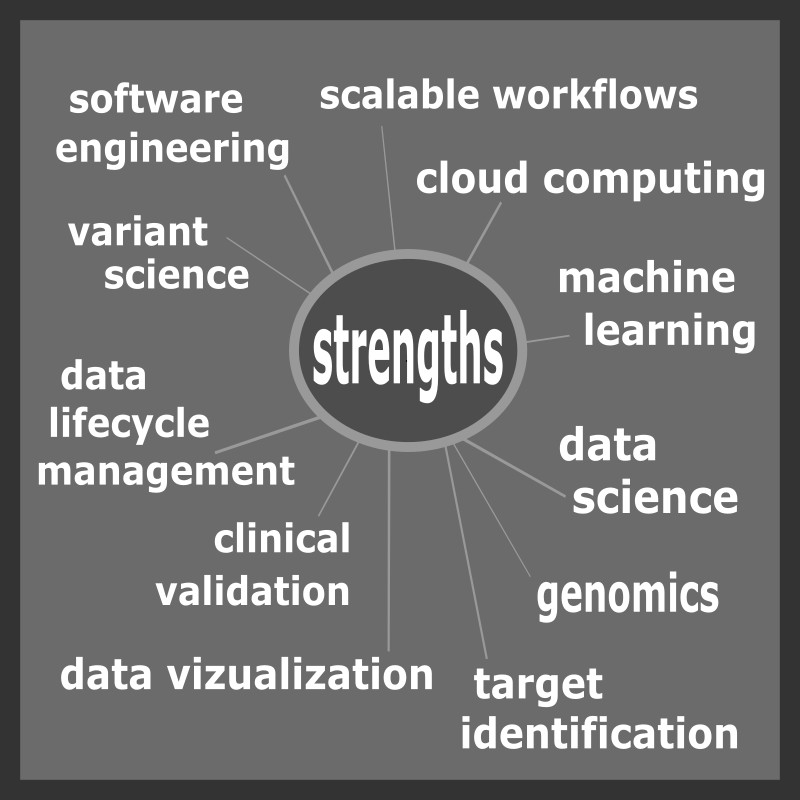
\includegraphics[scale=0.35]{expertise_sticknball.jpg}
\end{minipage}
\hfill
\begin{minipage}[c]{0.64\linewidth}
%bullet points of key info to right of image
	\begin{itemize}
	\small
	\item[$\bullet$] \textbf{Established and managed a highly-effective clinical bioinformatics group developing and supporting diverse systems with diverse data}
	\item[$\bullet$] \textbf{Wide breadth of experience both contributing and leading development of extensible, scalable software integrating big data with varied, complex data sets}
	\item[$\bullet$] \textbf{Deep expertise dedicated to bioinformatics research and engineering towards analysis, assay development, validation and clinical operations for diagnostic genetic testing}
	\item[$\bullet$] \textbf{Designed and implemented containerized cloud pipelines and supporting systems integrated into full end-to-end workflows}
	\item[$\bullet$] \textbf{Effective in the analysis and visualization of data.  I have significant ability to manage, transform, and distill data sets} 
	\item[$\bullet$] \textbf{I communicate in a way that makes technical concepts digestable to a variety of audiences}
%	\item[$\bullet$] \textbf{Skilled on a Linux command-line.  I can transform, merge, and distill information from big data in a distributed environment.}
%	\item[$\bullet$] \textbf{25 years experience applying bioinformatics in biotechnology, academic, and clinical settings}
%	\item[$\bullet$] \textbf{Strong in handling and processing next-generation sequence in scalable big-data environments}

       \end{itemize}
\end{minipage}
	\vspace*{0mm}
}}
    \vspace{-0pt}
\section{\Large{Education}}
  \resumeSubHeadingListStart
  
    % MAIN INFORMATION
    \resumeSubheading
    {University of Wisconsin-Madison}{Madison, WI}
    {Bachelors of Science, Botany}{1999}
        % BULLET POINTS
%        \resumeItemListStart
%            \resumeItem{\textbf{Selected Coursework:} COURSES}
%            \resumeItem{\textbf{Awards:} AWARDS}
%        \resumeItemListEnd
  \resumeSubHeadingListEnd
 \resumeSubHeadingListStart
         \resumeSubheading
    {Medical College of Wisconsin and Marquette University}{Milwaukee, WI}
    {Masters of Science, Joint Program in Bioinformatics}{2009}    
  \resumeSubHeadingListEnd


%%%%%%%%%%%%%%%%%%%%%%%%%%%%  Experience  %%%%%%%%%%%%%%%%%%%%%%%%%%%%
    \vspace{-0pt}
\section{\Large{Experience}}

    \resumeSubHeadingListStart
    
        % COMPANY 1
        \resumeSubheading
        {Quest Diagnostics}{Marlborough, MA}
            % POSITION 1
%            {\textbf{Sr. Manager, Bioinformatics}}{1/2018-Current}
            {\textbf{Sr. Staff Scientist/Sr. Manager, Bioinformatics}}{1/2018-Current}
            \resumeItemListStart
            	\resumeItem{Established and managed a highly skilled, high-functioning clinical bioinformatics group in development and in support of geneticists, variant scientists and lab operations as part of a highly-regulated genetic testing laboratory}
            	\resumeItem{Led and contributed to extensible, scalable software integrating core analyses with all systems required in our end-to-end sample processing workflow}
            	\resumeItem{Dedicated research and engineering towards primary analysis, assay development, validation and clinical operations}
            \resumeItemListEnd
            \hspace{5pt} Projects developed from initial research through implementation, validation, and in clinical operations:
            \resumeItemListStart
            	\resumeItem{Built first-in-kind long-read sequencing assay for quantification of tandem repeats using a CRISPR/Cas9 no-amp cleavage}
            	\resumeItem{Extensive development of containerized, cloud-based high-throughput analysis pipelines and integrating systems for large scale, consumer-based assay processing 100,000 samples over a year}
            	\resumeItem{Performed key analyses contributing to actionable insights and algorithms applied to complex data sets in support of multiple labs with varied workflows}
            	\resumeItem{Led development for high volume cloud-based systems and the tools to register and find data, track provenance, and ease troubleshooting of cloud pipelines and supporting systems}
            	\resumeItem{Drove extensible implementation of group’s Python libraries to standardize logging, tracking, and connection between LIMS, cloud-based systems and interpretation and reporting databases}
            	\resumeItem{Fostered extensibility and simplicity in all of the systems used in our production clinical setting}
            	
            	
%                \resumeItem{Built first-in-kind long-read sequencing assay for quantification of tandem repeats using a CRISPR/Cas9 no-amp cleavage}
%                \resumeItem{Built containerized, cloud-based high-throughput whole exome pipeline for large scale consumer-based assay processing 100,000 samples per year}
 %               \resumeItem{Established the systems needed to scale from small targeted panel assays to assays using a Whole Exome Sequencing backbone for diagnostic use}
%                \resumeItem{Produced Whole Exome Sequencing Copy Number Variant caller using a coverage-based approach}
%                \resumeItem{Established a dedicated Clinical Bioinformatics group in support of clinical geneticists, variant scientists and lab operations within a CAP/CLIA regulatory setting}
%                \resumeItem{Led development for high volume cloud-based systems and the tools to register and find data, track provenance, and ease troubleshooting of cloud pipelines and supporting systems}
 %               \resumeItem{Drove extensible implementation of group's Python libraries to standardize logging, tracking, and connection between LIMS, cloud-based systems and interpretation and reporting databases}
 %               \resumeItem{Fostered extensibility and simplicity in all of the systems used in our production clinical setting}
%%            \resumeItemListEnd
            % POSITION 2
%            \resumeSubheadingContinue
%            {\textbf{Sr. Staff Scientist, Bioinformatics, Research \& Development}}{}
 %%            \resumeItemListStart
            \resumeItemListEnd
  

        % COMPANY 2
        \resumeSubheading
        {Courtagen Life Sciences}{Woburn, MA}
            % POSITION 1
            {\textbf{Clinical Bioinformatics Scientist, Annotation \& Interpretation}}{11/2015-7/2017}
            \resumeItemListStart
                \resumeItem{Supported and implemented of interpretation and reporting full stack web applications providing feature improvements and Lifecycle Management in a CAP/CLIA genetic testing environment}
                \resumeItem{Built web interfaces and backends to identify and queue confirmatory analysis for diagnostic purposes}
            \resumeItemListEnd

    \resumeSubHeadingListEnd

%page end
\clearpage

%start new page
    \begin{center}
        % NAME
        {\Huge\scshape Jason J. Evans} 
        % SUBHEADING
        \\Bioinformatics Engineering and Data Science\\
        \small
        % EMAIL
        \href{mailto:jason.j.evans@gmail.com}{\raisebox{-0.2\height}\faEnvelope\  \underline{jason.j.evans@gmail.com}} ~ 
        % LINKEDIN
        \href{https://www.linkedin.com/in/jasonjevans/}{\raisebox{-0.2\height}\faLinkedin\ \underline{linkedin.com/in/jasonjevans}}  ~
        % GITHUB
        \href{https://github.com/jjevans}{\raisebox{-0.2\height}\faGithub\ \underline{github.com/jjevans}} ~
		%phone
		\href{tel:12624420503}{\raisebox{-0.2\height}\faPhone\ \underline{262-442-0503}}
    \end{center}
    
    
\vspace{-5pt}
\section{\Large{Experience (con'd)}}
    \resumeSubHeadingListStart
         % COMPANY 3
        \resumeSubheading
        {Laboratory of Molecular Medicine/Partners Personalized Medicine}{Cambridge, MA}
            % POSITION 1
            {\textbf{Clinical Bioinformatician}}{9/2012-11/2015}
            \resumeItemListStart
                \resumeItem{Produced end-to-end pipeline for distributed computation and variant calling for Whole Genome Sequencing in a CAP/CLIA genetic testing laboratory setting}
                \resumeItem{Implemented software to interface variant databases, variant annotation, and interpretation interfaces into a single, simple set of tools and resources}
            \resumeItemListEnd
   
        % COMPANY 4
        \resumeSubheading
        {Harvard School of Public Health, Bioinformatics Core}{Boston, MA}
            % POSITION 1
            {\textbf{Bioinformatician}}{7/2011-8/2012}
            \resumeItemListStart
                \resumeItem{Provided bioinformatics analyses and reports in support of contracting labs throughout HSPS}
                \resumeItem{Extensive contribution of tools and workflows towards the HSPS fork of the Galaxy Project}
            \resumeItemListEnd

        % COMPANY 4
        \resumeSubheading
        {Marquette University, School of Biology}{Milwaukee, WI}
            % POSITION 1
            {\textbf{Research Associate, Molecular Biology}}{5/2007-1/2008}
            \resumeItemListStart
                \resumeItem{Built molecular biology constructs for RNA Interference in \textit{Chlamydomonas}}
            \resumeItemListEnd


        % COMPANY 5
        \resumeSubheading
        {Applied Biosystems}{Foster City, CA}
            % POSITION 1
            {\textbf{Bioinformatics Scientist, Research \& Development}}{5/2001-5/2005}
            \resumeItemListStart
                \resumeItem{Built the computational analysis and system to run it in support of SNPlex custom oligo array}
                \resumeItem{Assisted in development of the first ABI 7900 high-throughput qPCR platform.  Provided continued improvements in basecalling for the ABI 3700 sequencing instrument}
				\resumeItem{Leveraged the Celera human genome draft to identify putative drug targets in collaboration with contracted pharmaceutical companies}
            \resumeItemListEnd   
            
        % COMPANY 6
        \resumeSubheading
        {Celera Genomics}{Foster City, CA}
            % POSITION 1
            {\textbf{Scientist}}{5/2000-5/2001}
            \resumeItemListStart
                \resumeItem{Wet lab identification of full-length cDNA clones targeting putative drug targets}
                \resumeItem{cDNA library archival in a high-throughput cloning laboratory focused on isolating drug targets identified by draft genome}
            \resumeItemListEnd   
    \resumeSubHeadingListEnd

%%%%%%%%%%%%%%%%%%%%%%%%%%%%  Publications  %%%%%%%%%%%%%%%%%%%%%%%%%%%%
\vspace{-5pt}
\section{\Large{Publications}}
	\begin{itemize}[leftmargin=0.15in, label={}]
		\small{\item{Tsai, E.A.; Shakbatyan, R.; Evans, J.; Rossetti, P.; Graham, C.; Sharma, H.; Lin, C.-F.; Lebo, M.S. \textbf{Bioinformatics Workflow for Clinical Whole Genome Sequencing at Partners HealthCare Personalized Medicine}. J. Pers. Med. 2016, 6, 12.}}
	\end{itemize}


%outline box
%%\vspace*{-0.75in}

\vspace{0pt}
%\section{\Large{Attributes}}
\section{}
   \vspace{-0pt}
\begin{minipage}[c]{0.5\linewidth}
\fbox{\parbox{\linewidth}{ 
\begin{flushleft}\Large{\textbf{Technical Skills}}\end{flushleft}
   \begin{itemize}
    [leftmargin=0.15in, label={}]\small{\item{
        \textbf{Sequencing}{: PacBio Long-read, NGS Whole Exome, Whole Genome} \\
        \textbf{Stats \& Data Science}{: R, Bioconductor\\ ggplot2/dplyr/tidyverse, Pandas, Plotly} \\
        \textbf{Machine Learning}{: scikit-learn, PyTorch} \\
        \textbf{Languages}{: Python, Ruby, Java, Javascript, CSS, SQL} \\
        \textbf{AWS}{: S3, API Gateway, IAM, ECR, Lambda, EC2, Batch} \\
        \textbf{Containerization}{: Docker, Rancher } \\        
        \textbf{Variant Calling}{: Small, Copy Number, Structural, Tandem repeat variation} \\
        \textbf{Databases}{: Relational, NoSQL, Document} \\
        \textbf{Regulatory}{: College of American Pathology (CAP), CLIA} \\
        \textbf{Environments}{: Conda, Jupyter} \\        
        \textbf{Web Frameworks}{: Flask, FastAPI, VueJS} \\        
%        \textbf{Package Installers}{: Conda, pip, yum/apt, npm} \\
%        \textbf{Workflow Languages}{: WDL, DNAnexus, Nextflow} \\
    }}
    \end{itemize}}
}
\end{minipage}
\vspace{-0mm}
\hfill
\vspace{10mm}
\begin{minipage}[top][3.25in][]{3in}
%	
%	\begin{mybox}{Cloud Computing}{\faIcon[regular]{check-square}}{gray!95!black}
%		Extensive experience in containerization and processing in AWS
%	\end{mybox}
%	\begin{mybox}{Data Visualization}{\faIcon[regular]{check-square}}{gray!95!black}
%		Exceptional at data extraction, analysis, and chart generation
%	\end{mybox}
%	\begin{mybox}{Infrasture Capability}{\faIcon[regular]{check-square}}{gray!70!black}
%		Strong capability in cloud, on-premise, and hybrid linux infrastructure
%	\end{mybox}
%	\begin{mybox}{Genetics and Genomics}{\faIcon[regular]{check-square}}{gray!95!black}
%		Deep understanding of genetics along with the genomic tools to use it
%	\end{mybox}
%%	\begin{mybox}{Commitment}{\faIcon[regular]{hand-peace}}{gray!70!black}
%	\begin{mybox}{Commitment}{\faIcon[regular]{check-square}}{gray!70!black}
%		I value personal growth in myself and others.  I promote a dynamic team.
%	\end{mybox}
%\end{minipage}
%\begin{minipage}{0.4\linewidth}
%   \vspace{4mm}
%	\begin{mybox}{Lead by Example}{\faIcon[regular]{cog}}{gray!95!black}
%		Initiative and work ethic shows the way we do business.
%	\end{mybox}
%	\begin{mybox}{Lead by Conversation}{\faIcon[regular]{lightbulb}}{gray!70!black}
%		Pursue by question and direct by answer.  It promotes a dynamic team.
%	\end{mybox}
%	\begin{mybox}{Lead by Coaching}{\faIcon[regular]{handshake}}{gray!95!black}
%	Investment in personal growth returns strength, skills and understanding.
%	\end{mybox}
%	\begin{mybox}{Lead by Transformation}{\faIcon[regular]{lightbulb}}{gray!70!black}
%		Inspire by growing ourselves into\\ our own future.
%	\end{mybox}
%\end{minipage}

%%functional 4 boxes.
%%\noindent\framebox{\begin{tikzpicture}
%%\node [tikzbox, align=left] (a) at (0,0) {\small{\textbf{Sequencing}\\PacBio long-read\\Whole Exome\\Whole Genome\\Microarray\\qPCR\\\textbf{Genetic Testing}\\Direct-to-consumer\\LDT}};
%%\node [tikzbox, align=left] (b) at (0,-4) {\small{\textbf{Infrastructure}\\AWS\\LIMS\\Docker/Rancher\\FastAPI/Flask\\Conda\\JupyterLab\\Nextflow/WDL}};
%%\node [tikzbox, align=left] (c) at (4,0) {\small{\textbf{Technologies}\\Python\\Javascript\\CSS\\Ruby\\R\\Bioconductor\\tidyverse/ggplot2}};
%%\node [tikzbox, align=left] (d) at (4,-4) {\small{\textbf{Variant Calling/\\Markers}\\Germline\\Somatic\\Joint/Relatedness\\Copy Number\\Structural\\Tandem Repeat}};
%%\end{tikzpicture}}
%\hfill
%%%%%\begin{minipage}[top][4.5in][]{4in}
    \vspace{-0in}
	\begin{mybox}{Cloud Computing}{\faIcon[regular]{check-square}}{gray!95!black}
		Extensive experience in containerization and processing in AWS
	\end{mybox}
	\begin{mybox}{Data Science}{\faIcon[regular]{check-square}}{gray!95!black}
		Exceptional at data extraction, analysis, and chart generation
	\end{mybox}
%	\begin{mybox}{Infrasture Capability}{\faIcon[regular]{check-square}}{gray!70!black}
%		Strong capability in cloud, on-premise, and hybrid linux infrastructure
%	\end{mybox}
	\begin{mybox}{Genetics and Genomics}{\faIcon[regular]{check-square}}{gray!95!black}
		Deep understanding of genetics along with the genomic tools to use it
	\end{mybox}
%	\begin{mybox}{Commitment}{\faIcon[regular]{hand-peace}}{gray!70!black}
%	\begin{mybox}{Commitment}{\faIcon[regular]{check-square}}{gray!70!black}
%		I value personal growth in myself and others.  I promote a dynamic team.
%	\end{mybox}	
	\begin{mybox}{Algorithm Development}{\faIcon[regular]{check-square}}{gray!70!black}
		Wide breadth in statistical analysis, machine learning, and software
	\end{mybox}
\end{minipage}




\end{document}
